\documentclass{report}
\usepackage{float}

% for the image in the title
\usepackage{tikz}

% custom spacing
\usepackage{setspace}
\onehalfspacing

% footer and header
\usepackage{fancyhdr}
% \setlength{\headheight}{15.2pt}

% underlining
\usepackage{ulem}

\usepackage[T1]{fontenc}

% Table of contents link to corresponding sections
\usepackage{hyperref}
\hypersetup{
	colorlinks,
	citecolor=black,
	filecolor=black,
	linkcolor=black,
	urlcolor=black
}

\usepackage{amsmath}
% Remove che "Chapter" string before chapters
\iffalse
\makeatletter
\def\@makechapterhead#1{%
	\vspace*{50\p@}%
	{\parindent \z@ \raggedright \normalfont
		\interlinepenalty\@M
		\Huge\bfseries  \thechapter.\quad #1\par\nobreak
		\vskip 40\p@
}}
\makeatother
\fi

% Fancy chapters
\usepackage[Bjarne]{fncychap}
% options: Sonny, Lenny, Glenn, Conny, Rejne, Bjarne, Bjornstrup

\begin{document}
	
	
	%title page
	\begin{titlepage}
		\begin{figure}[t]
			\centering
\includegraphics[width=0.3\textwidth]{images/unitn-logo}
		\end{figure}
		\begin{center}
			\textsc{ \LARGE{Università degli Studi di Trento \\}}
			\textsc{ \LARGE{Facoltà di Informatica\\ }}
			\textnormal{ \LARGE{Corso di Ingegneria del Software\\}}
			\vspace{30mm}
			\fontsize{10mm}{7mm}\selectfont 
			\textup{FixMi \\ Report Finale}\\
		\end{center}
		
		\vspace{25mm}
		
		\centering
		\large Gruppo G43: \\ Giovanni Santini\\ Riginel Ungureanu \\ Valerio Asaro
		
		\vspace{20mm}
		
		\centering{\large{Anno Accademico 2023/2024 \\ Trento }}
		
	\end{titlepage}
	
	
	
	
	% use header and footers
	\pagestyle{fancy}
	\fancyhead[R]{\chaptername\ \thechapter}  % header
	
	%\maketitle
	\tableofcontents
	\newpage
	
	
	
	\section{Scopo del documento}
	
	Il seguente documento contiene una valutazione finale del processo e l'organizzazione per lo sviluppo dell'applicazione "FixMi".
	
	\section{Informazioni del Documento}
	
	% table
	\begin{center} % center the table
		\centering
		\begin{tabular}{ |p{4cm}|p{4cm}|  }
			\hline
			\centering Campo & \qquad\qquad Valore \\ % I found no other way...
			\hline
			Titolo del Documento & Report Finale \\
			\hline
			Titolo del Progetto & FixMi \\
			\hline
			Autori del Documento &
			Giovanni Santini \\ & Riginel Ungureanu \\ & Valerio Asaro \\
			\hline
			Amministratore Progetto & Riginel Ungureanu\\
			\hline
			Versione del documento & 1.1 \\
			\hline
		\end{tabular}
	\end{center}
	
	
	
\chapter{Report}

\section{Approcci all'ingegneria del software}

\subsection{Blue Tensor}
\subsubsection*{Riassunto}
L'ingegnere Jonni Malacarne inizia la presentazione raccontando la nascita di "Blue Tensor", un'azienda nata a Firenze nel 2018 che si pone come obiettivo lo sviluppo di prodotti basati sull'intelligenza artificiale in ambito industriale. Il principale punto di forza di Blue Tensor, sottolinea l'ingegnere, è la forza di coesione del team di sviluppo in quanto affrontare progetti di grandi dimensioni può risultare talvolta complicato.
Dopo aver mostrato alcuni prodotti offerti da Blue Tensor, con particolare attenzione per la "Computer Vision", il CEO continua il suo discorso spiegando l'approccio adottato dal suo team per lo sviluppo del software. Una dettagliata composizione del gruppo lavorativo, dotato di ruoli ed occupazioni ben specifiche, viene poi seguito da una "RoadMap" dell'intero progetto, rendendo l'intera produzione più fluida e semplice da gestire. Blue Tensor, in particolare, adotta un approccio a cascata, formato da 6 "Work Packages":
\begin{itemize}
	\item WP0: PMO and Quality Assurance
	\item WP1: Analisi e Fattibilità
	\item WP2: Setup e Design
	\item WP3: Data Preparation
	\item WP4: Sviluppo, Training, Test, Deploy
	\item WP5: Rilascio Finale
\end{itemize}
Il CEO conclude la presentazione con una lista di strumenti ingegneristici per l'analisi e la comunicazione del cliente che il team di Blue Tensor utilizza:
\begin{itemize}
	\item UML
	\begin{itemize}
		\item Use Case Diagrams
		\item Activity Diagrams
		\item State Machine Diagrams
		\item Architecture Diagrams
	\end{itemize}
	\item E-R per i DataBase
	\item Mockups - per il design UI 
	\begin{itemize}
		\item Low-Fidelity Mockups
		\item High-Fidelity Mockups
	\end{itemize}
	\item Prototipi
	\item Mappe Mentali
\end{itemize}

\subsubsection*{Cosa abbiamo imparato}
Abbiamo imparato che il primo passo per il raggiungimento di un obiettivo è un'ottima squadra di sviluppo, che sappia individuare i propri punti di forza ma anche di debolezza e che sappia agire di conseguenza. Come secondo passo, invece, c'è una rigorosa pianificazione dal punto di vista organizzativo del progetto, cercando di non lasciare niente al caso.

\subsubsection*{Il nostro approccio}
Il nostro team ha agito in linee molto simili a quelle presentate dal CEO di Blue Tensor: anche noi abbiamo individuato dei ruoli nella nostra squadra, ci siamo organizzati in base a questi ultimi ed abbiamo suddiviso in maniera equa ed intelligente il lavoro rispettando i limiti di ogni singolo individuo all'interno del gruppo.


\subsection{Kanban}
\subsubsection*{Riassunto}

Il seminario ha mostrato, tramite un laboratorio interattivo, le potenzialità del metodo Kanban. Nonostante il termine Kanban venga utilizzato del mondo automobilistico, nell'informatica Kabnan è un metodo per gestire il lavoro utilizzato da molte aziende come Microsoft durante lo svilupo di X-box. Il metodo si basa sulla divisione del lavoro in diverse sezioni, come "Design", "Implementation" e "Done". Una certa task passerà tramite queste fasi di sviluppo, in modo da fornire una visione chiara dello stato di una task. kanban si basa sul fatto che ci può essere un numero limitato di task su cui si sta lavorando contemporaneamente. Questo permette di concentrare l'intero team su un unico obiettivo e completare tasks più in fretta. Lo scopo del laboratorio è stato mostrare come questo sistema funziona.

\subsubsection*{Cosa abbiamo imparato}

Un sistema di gestione del lavoro è fondamentale per un processo di sviluppo efficiente e produttivo. Kanban fornisce un metodo di organizzare il lavoro per questi scopi.

\subsubsection*{Il nostro approccio}

Anche se non è stato usato il metodo Kanban, durante lo sviluppo il team ha diviso il lavoro in più task e si è concentrato su un obiettivo alla volta.

\subsection{IBM}
\subsubsection*{Riassunto}
Il seminario viene  presentato dal Cloud Technical Specialist Ferdinando Gorga di IBM.
Comincia presentandoci i servizi cloud di IBM, i diversi livelli di astrazione dal bare metal al serverless, e i vantaggi della piattaforma.
Procede facendo l'esempio di un'architettura molto vulnerabile, e i vari metodi per migliorarla utilizzando tecnologie cloud.
Successivamente ci mostra il catalogo di IBM cloud, dove è possibile acquistare varie componenti che funzionano tra di loro senza problemi, per poi mostrarci il code engine, che è alla base del serverless. Una particolarità è la load distribution, in quanto le istanze dell'applicazione si moltiplicano e dividono in base al carico,
arrivando perfino a spegnersi in caso di mancanza di traffico. 
Inoltre ci mostra un semplice linguaggio di scripting grafico nominato NodeRED.

Infine ci mostra il concetto di Cloud Satellite: Un modo per integrare i propri computer e server all'interno dell'ecosistema cloud di IBM.
\subsubsection*{Cosa abbiamo imparato}
Abbiamo imparato quanto sia importante il cloud al giorno d'oggi, in quanto i giusti servizio e tecnologie permettono di dedicarsi al codice e non all'infrastruttura sottostante.
\subsubsection*{Il nostro approccio}
Il deploy non lo abbiamo fatto su nessuna piattaforma di cloud, tuttavia abbiamo seguito l'approccio dei container per i nostri microservizi. 
Grazie a ciò non soffriamo di problemi di compatibilità tra le macchine, il software è portabile e siamo certi che con un po' di lavoro si potrebbe rilasciare sul cloud.

\subsection{META}
\subsubsection*{Riassunto}
L'ingegnere del software Heorhi Raik presenta la sua esperienza all'interno di "META", una delle più grandi aziende informatiche del mondo. Dopo aver raccontato brevemente i suoi studi, la sua carriera e il suo ruolo all'interno dell'azienda, pone grande attenzione sui ruoli lavorativi che META propone:
Solitamente, dopo una serie di colloqui in cui l'attenzione viene posta più sulle capacità di pensiero critico e logico dell'individuo piuttosto che sulla conoscenza di specifici linguaggi di programmazione, si inizia il proprio percorso all'interno di "META" con il titolo di "Junior": il tipico programmatore addetto alla scrittura e produzione di codice. Dopo qualche anno, tuttavia, il ruolo di "Junior" si evolve in "Senior". L'importanza dell'individuo all'interno dell'azienda aumenta, in quanto adesso può essere a capo di gruppi di sviluppo, di progetti o addirittura di interi dipartimenti. È chiaro, quindi, che le capacità richieste al tipico "Senior" sono organizzative e di pianificazione, caratteristiche di un vero e proprio "Ingegnere del Software".
La presentazione si conclude con una breve parentesi sugli strumenti di sviluppo utilizzati all'interno di META.

\subsubsection*{Cosa abbiamo imparato}
Entrare a far parte di un'azienda di grande importanza come "META" non richiede necessariamente abilità in specifici linguaggi di programmazione o particolari modi di scrivere codice. Anzi, si potrebbe far parte di un colosso dell'informatica scrivendo solo una o due righe di codice al giorno: il ruolo di leader del gruppo può essere talvolta più complicato e impegnativo. Proprio per questo, non bisogna sottovalutare il ruolo di "Software Engineer", in quanto ha le abilità necessarie per potersi porre a capo di un eventuale team di sviluppo.

\subsubsection*{Il nostro approccio}
All'interno del nostro gruppo abbiamo posto grande attenzione nella scelta del leader, considerando la quantità di conoscenze possedute ma soprattutto le capacità amministrative e organizzative. Questo ha sicuramente reso il percorso di sviluppo più semplice e meno tortuoso.


\subsection{U-Hopper}

\subsubsection*{Riassunto}

Daniele Miorandi, Chief AI Officer  di U-Hopper, ha dedicato il seminario per familiarizzare gli studenti con tecnologie utilizzate in azienda, portando l'esempio di U-Hopper. Le tecnologie mostrate sono le seguenti:
\begin{itemize}
	\item \textbf{Ingestion}: Per reperire grandi quantità di dati, vengono utilizzati dei sistemi a coda come dei buffers e dei lettori e scrittori. Esempi di queste tecnologie sono Kafka, MQTT
	\item \textbf{Batch Processing}: Computazione in blocchi su cluster. Esempio di Spark.
	\item \textbf{Stream Processing}: Elaborazione dei dati in streams, spesso usati nei sistemi di pagamento. alcune tecnologie sono Spark Streaming e Flink
	\item \textbf{In-memory DB}: Tenere tutti i dati in memoria per una maggiore velocità di lettura. Esempio: Redis
	\item \textbf{Storage}: PostgeSQL, MongoDB, MySQL, Cassandra (Per grandi dati molto sparsi, inserisce per colonne), CouchDB, Elastic (NpSQL per letture e scritture veloci), InfluxDB (lavoro per serie temporali come dati di sensori e logs), MinIO (Object storage), TileDB(gestione di dati cartografici)
	\item \textbf{Task Management / Orchestration}: Tecnologie per controllare l'esecuzione e i flow dei dati, rappresentati tramite DAG. Ad esempio Celery e AirFlow
	\item \textbf{Logs}: Sentry, ELK, TIG
	\item \textbf{Linguaggi di programmazione}: Python, Scala, go
	\item \textbf{AI}: MLFlow, Tenserflow, Pythorch
	\item \textbf{DEployment}: Docker, IASS
	\item \textbf{DEsign Patterns}: Microservizi, Event Driven Architecture, Asynchronous
	\item \textbf{Processi e strumenti per SE}: Agile, CI / CD, documentazione
\end{itemize}

\subsubsection*{Cosa abbiamo imparato}

Esistono numerose tecnologie per la realizzazione di software utilizzate in azienda. Queste tecnologie permettono di risolvere problemi o migliorare il processo di sviluppo. 

\subsubsection*{Il nostro approccio}

Nella creazione dello stack per la nostra applicazione, abbiamo tenuto conto delle tecnologie più utilizzate nell'industria compatibili con i nostri requisiti ed esperienza. Abbiamo utilizzato un design pattern basato sui microservizi ed una serie di tecnologie utili allo sviluppo come linters, tests, agile developement.

\subsection{RedHat}

\subsubsection*{Riassunto}
Il seminario, presentato da Mario Fusco di RedHat, introduce il mondo dell'open source e delle sue dinamiche. Vengono elencati i vantaggi nell'open source quali la condivisione di conoscenza, il controllo del codice da molti e la community. Vengono discusse le licenze, divise nelle due categorie Copyleft e non-Copyleft. La prima forza la distribuzione del codice delle applicazioni modificate dall'originale, la seconda non obbliga nessuna restrizione sull'utilizzo del codice. Il seminario si conclude mostrando come poter contribuire ad un progetto open source, principalmente guardando la sezione "Issues" su github.
\subsubsection*{Cosa abbiamo imparato}
L'open source è un ottimo sistema per lo svuiluppo di software sotto tanti aspetti.


\subsection{Microsoft}
\subsubsection*{Riassunto}
Il seminario viene presentato dal Senior Software Engineer Diego Colombo.
Comincia presentandoci il concetto di testing, i suoi utilizzi e i vari tipi, e usa come esempio particolare l'acceptance testing e il behaviour driven development(bdd).
Successivamente ci spiega perchè è importante testare e perchè sono fondamentali degli health check all'interno di un'architettura a microservizi.
Dopodichè dimostra i vari tipi di tool per il testing - dal Unit Test framework ai test runner continui, 
per poi dirci che i test vengono idealmente svolti in diversi contesti e diverse fasi: Nella macchina di sviluppo, nell'environment di build, in production e perfino nel computer dell'utente finale.
Ci mostra degli esempi di strumenti di testing scrivendo il codice in tempo reale:
\begin{itemize}
	\item Mocha, framework di test e Chai, framework di asserzioni 
	\item Wallaby, un test runner continuo e con supporto di live comment
	\item Playwright, che simula un browser per testare le funzionalità di ui e permette di fare mocking
\end{itemize}
Infine ci spiega la filosofia del Test Driven Development, dove i test vanno scritti ancora prima del codice.
\subsubsection*{Cosa abbiamo imparato}
Questo seminario ci ha fatto capire l'importanza dei test e il modo in cui la loro presenza possa facilitare lo sviluppo. Inoltre il test driven development è un approccio interressante che sicuro adotteremo in futuri progetti. 
\subsubsection*{Il nostro approccio}
Per il testing delle nostre API abbiamo usato Jest, molto simile a Mocha, e Supertest, ottima per testare le richieste http. Non abbiamo seguito un approccio TDD, però abbiamo messo grande importanza nel testing di ogni API.

\subsection{Molinari}
\subsubsection*{Riassunto}
Il Professore Andrea Molinari presenta il settore "Legacy", quel particolare settore informatico caratterizzato dalla presenza di elementi Hardware, Software, Reti, Dati e Processi "obsoleti", cioè aventi prestazioni e caratteristiche di gran lunga superate e migliorate, ma che sono ancora in uso.
Il mondo legacy coinvolge maggiormente il mondo delle grandi società informatiche, società che quindi hanno effettuato un grande investimento in "Mainframes" e "Super sistemi" difficili da rimpiazzare o migliorare con facilità.Stiamo parlando di sistemi aventi in media:
\begin{itemize}
	\item Server da 240 CPU
	\item 40 TeraByte di RAM
	\item Dischi di persistenza dalle dimensioni di PetaBytes
\end{itemize}
Il professore sottolinea il problema del mondo "Legacy" da un punto di vista della produzione del software, più che del rimpiazzamento hardware:
I linguaggi utilizzati per la realizzazione dei programmi diventano velocemente obsoleti, esempio noto "Cobol": un linguaggio ancora oggi ampiamente utilizzato e che sta alla base di quasi tutte le transazioni economiche globali.
Non solo, ma cambiare radicalmente tecnologia dall'oggi al domani è altamente rischioso per una qualsiasi azienda, questo per 4 semplici motivi:
\begin{itemize}
	\item Continuità: "Se funziona, perchè dovrei rimpiazzarla?"
	\item Ambiguità: "Visto che stiamo rinnovando il sistema, miglioriamo questa funzionalità, aggiungiamo quest'altra"
	\item Complessità del codice e della documentazione: E' quasi impossibile riscrivere  in pochi mesi un software che ha richiesto anni per essere realizzato.
	\item Recovery: Molte aziende ancora oggi tendono ad avere un cloud ibrido, cioè che hanno un mainframe privato per il backup in locale e anche nel cloud
\end{itemize}
Qualche soluzione, continua il professore, è possibile:
Ultimamente si sta sperimentando molto con delle Intelligenze Artificiali che possano riscrivere il codice obsoleto, velocizzando drasticamente il processo. Un altra soluzione potrebbe essere l'incapsulamento del vecchio sistema legacy all'interno di un nuovo sistema, sotto forma di componente.
L'ultima parte della presentazione è stata dedicata alla gestione organizzativa per un progetto legacy: il metodo AGILE qui fallisce miseramente in quanto:
\begin{itemize}
	\item Il progetto Legacy è molto grande, solitamente è il risultato di anni ed anni di modifiche e sviluppi
	\item Il Team legacy è un team complesso, composto da elementi di tutte le generazioni e di tutti i tipi. Molti ruoli diversi, impossibili da gestire con semplicità.
	\item La comunicazione con il cliente è complicata, se non del tutto inesistente: i progetti Legacy vedono solitamente protagonisti multisocietà formate da aziende di medio-grosso calibro: tante linee di pensiero impossibili da riunire in uno solo e con cui potere interloquire.
\end{itemize}

\subsubsection*{Cosa abbiamo imparato}
Abbiamo imparato che la produzione di codice e di documentazione non deve essere solo fine a se stessa e alla conclusione del progetto, ma deve anche dare un importante sguardo verso un futuro prossimo. Un futuro in cui potrebbe essere necessario tornare indietro per modificare o riscrivere parte dell'applicazione per portarla nuovamente agli standard del periodo.

\subsubsection*{Il nostro approccio}
La suddivisione della nostra applicazione in più microservizi rende l'intero progetto altamente scalabile e facile da modificare. Le tecnologie utilizzate per la realizzazione del progetto sono inoltre all'avanguardia per il nostro periodo, dunque non dovrebbero esserci problemi in un prossimo futuro.


\subsection{Marsiglia}
\subsubsection*{Riassunto}
Il seminario viene presentato dal Enterprise Architect Gerardo Marsiglia
Comincia presentandoci i vari ruoli all'interno di un progetto, quali Specialista, Architetto, Consulente, Ingegnere e Manager.
Ci parla del ciclo di vita del software che, soprattutto nei grandi e vari team di sviluppo, è difficile da gestire. E' fondamentale definire standard, organizzare lo sviluppo e utilizzare tool di automazione.
Successivamente ci parla dell'evoluzione delle metodologie di sviluppo, partendo da waterfall, passando a quelle iterative, all'Agile e infine al DevOps.
Dopodichè spiega il concetto di Continous Delivery, processo fondamentale del DevOps che si integra con il Continous Integration. 
Ciò che è più evidente è che il processo di Continous Delivery è spesso automatizzabile, il che velocizza tutto.
Successivamente parla di Modernizzazione Applicativa, un processo fondamentale per modernizzare le applicazioni tradizionali e ottenere i vantaggi delle nuove tecnologie.
In questo segmento parla anche dell'evoluzione dell'architettura software, partendo dal monolith per arrivare poi all'architettura a microservizi, e i vari livelli di astrazione dal Bare metal ai container.
Infine ci mostra l'esempio della domotizzazione di casa sua, dove ha utilizzato una soluzione open source per unire i vari dispositivi di diversi marchi in un' unica applicazione dalla quale controllarli.

\subsubsection*{Cosa abbiamo imparato}
Abbiamo imparato che la gestione del ciclo di vita è veramente importante e non va mai trascurato, ci ha offerto uno scorcio nel mondo del DevOps e in particolare del CI/CD.
\subsubsection*{Il nostro approccio}
Per il progetto non abbiamo seguito una metodologia precisa, tuttavia durante alcune fasi dello sviluppo del codice abbiamo seguito un approccio simile al Continous Integration.
Inoltre abbiamo sviluppato un'architettura a microservizi.

\subsection{APSS \& Trentino.ai}

\subsubsection*{Riassunto}
Il seminario discute le tencologie e il data flow utilizzati nell'Azienda Provinciale per i Servizi Sanitari (APSS). L'APSS segue un gran numero di dipendenti, professionisti e pazienti su tutto il territorio occupandosi della manutenzione delle attrezzature sanitarie e della gestione dei dati. Infatti vengono utilizzate diverse tecnologie per l'elaborazione e la visualizzazione dei dati come KNIME e Tableau. Inoltre, vi è un interesse nell'adozione di soluzioni basate su AI nel mondo della sanità.

\section{Organizzazione del lavoro}

Il team di sviluppo ha deciso di adottare una struttura organizzativa orizzontale: una struttura organizzativa in cui tutti i membri della squadra di sviluppo possiedono eque responsabilità.
% Il team ha adottato il seguente organigramma:
Avendo suddiviso il progetto in microservizi è stato possibile gestire la mole di lavoro in maniera asincrona, garantendo una fluidità lavorativa semplice ed efficace: la stesura della documentazione e la scrittura del codice sono state divise in modo equo tra i membri del team di sviluppo
in modo da poter lavorare in contemporanea.
A tale scopo il lavoro è stato diviso in macro obiettivi (rappresentati dai cinque deliverables) a loro volta suddivisi in obiettivi comuni (individuati dai capitoli di ciascun deliverable) e task individuali (rappresentate dalle contribuzioni di ciascun individuo al fine di completare l'obiettivo).
La realizzazione del lavoro è stata suddivisa, specialmente nell'ultimo periodo, in più sprints, dove il team di sviluppo si è impegnato a svolgere le proprie task individuali entro una scadenza ben precisa, concordata tra i membri stessi . Durante questi periodi il team si è riunito con frequenza settimanale per discutere riguardo lo stato del progetto, degli obiettivi in corso e quelli successivi.
Per l'organizzazione dello sviluppo il team ha adottato un Workflow basato sul Branching e sulle Pull Requests di GitHub: ogni membro ha lavorato alla propria versione del progetto, inviando le proprie modifiche agli altri membri del gruppo tramite la creazione di "Pull Requests": dopodichè viene effettuato, da parte degli altri membri, un controllo sulla qualità e la correttezza delle modifiche.
Il team di sviluppo ha fatto uso dei seguenti strumenti per lo sviluppo dell'applicazione

\begin{itemize}
	\item Trello
	\begin{itemize}
		\item Software collaborativo per la gestione e l'organizzazione del lavoro di un gruppo.
		\begin{figure}[H]
			\centering
			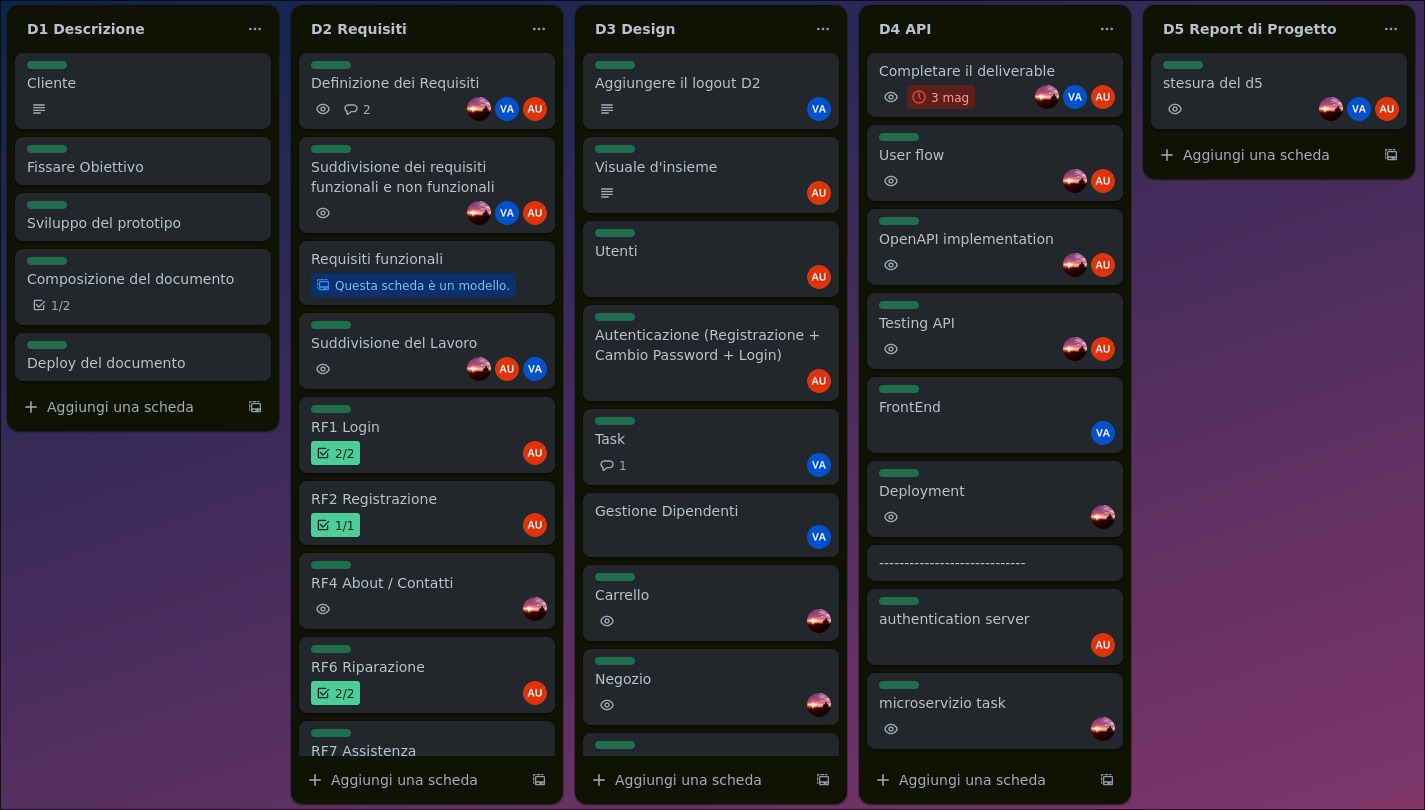
\includegraphics[width=1\textwidth]{images/trello-image.jpg}
			\caption{Organizzazione del lavoro su Trello}
		\end{figure}	
	\end{itemize}
	\item GitHub
	\begin{itemize}
		\item Piattaforma per lo sviluppo di software che permette di creare, immagazzinare, gestire e condividere il codice.
	    \begin{figure}[H]
	    	\centering
	    	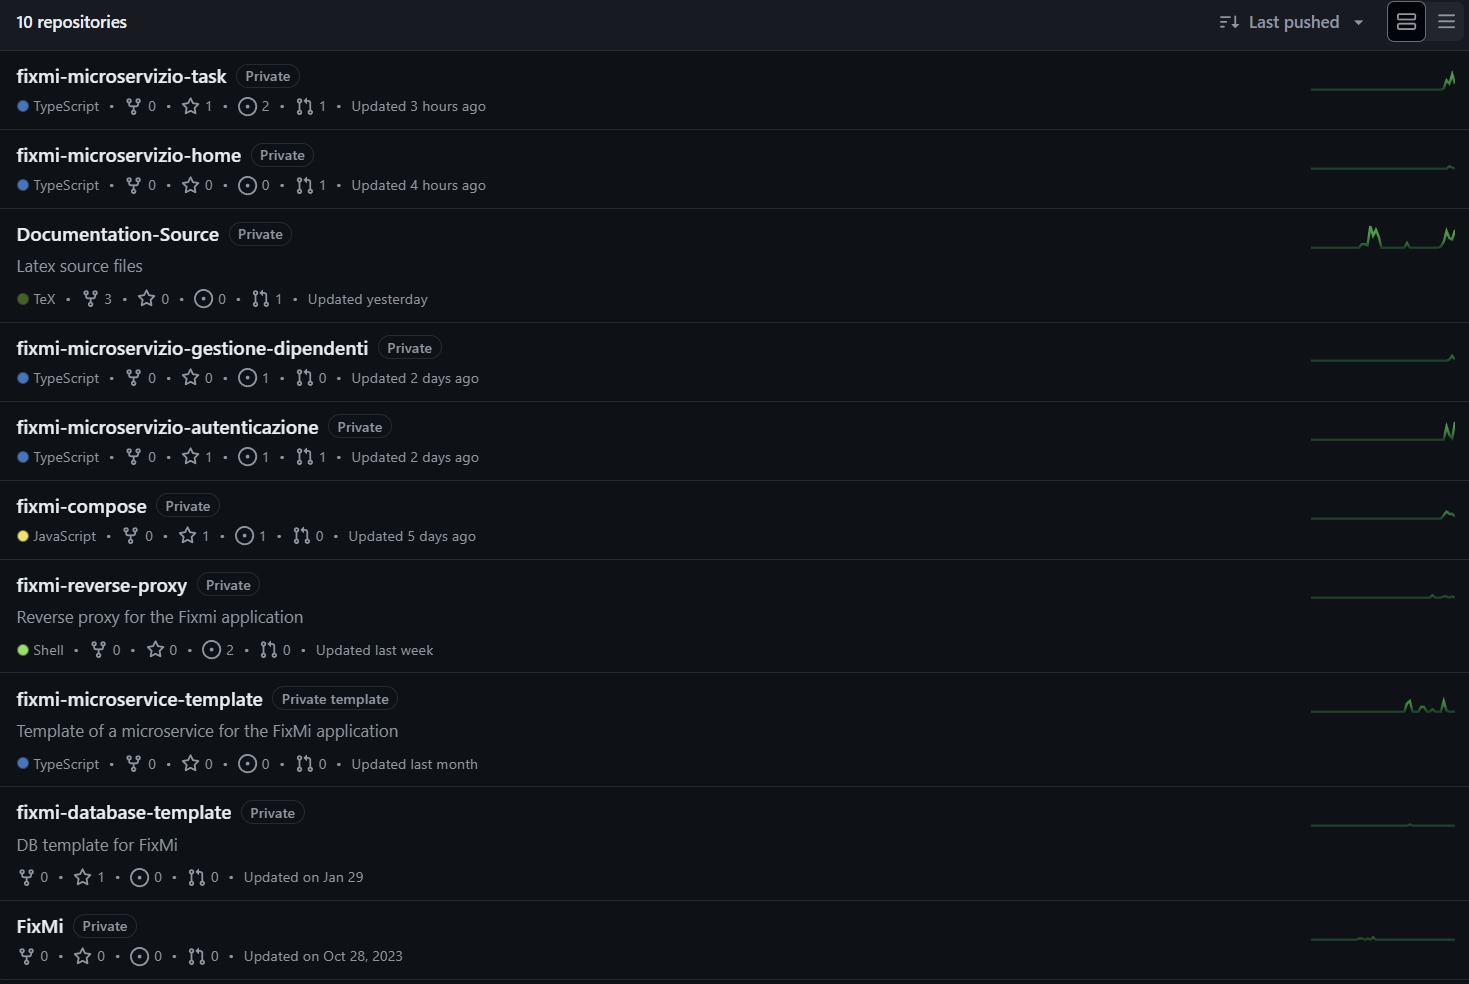
\includegraphics[width=1\textwidth]{images/github-image1.jpg}
	    	\caption{Organizzazione del progetto su GitHub}
	    \end{figure}	
	    \begin{figure}[H]
	    	\centering
	    	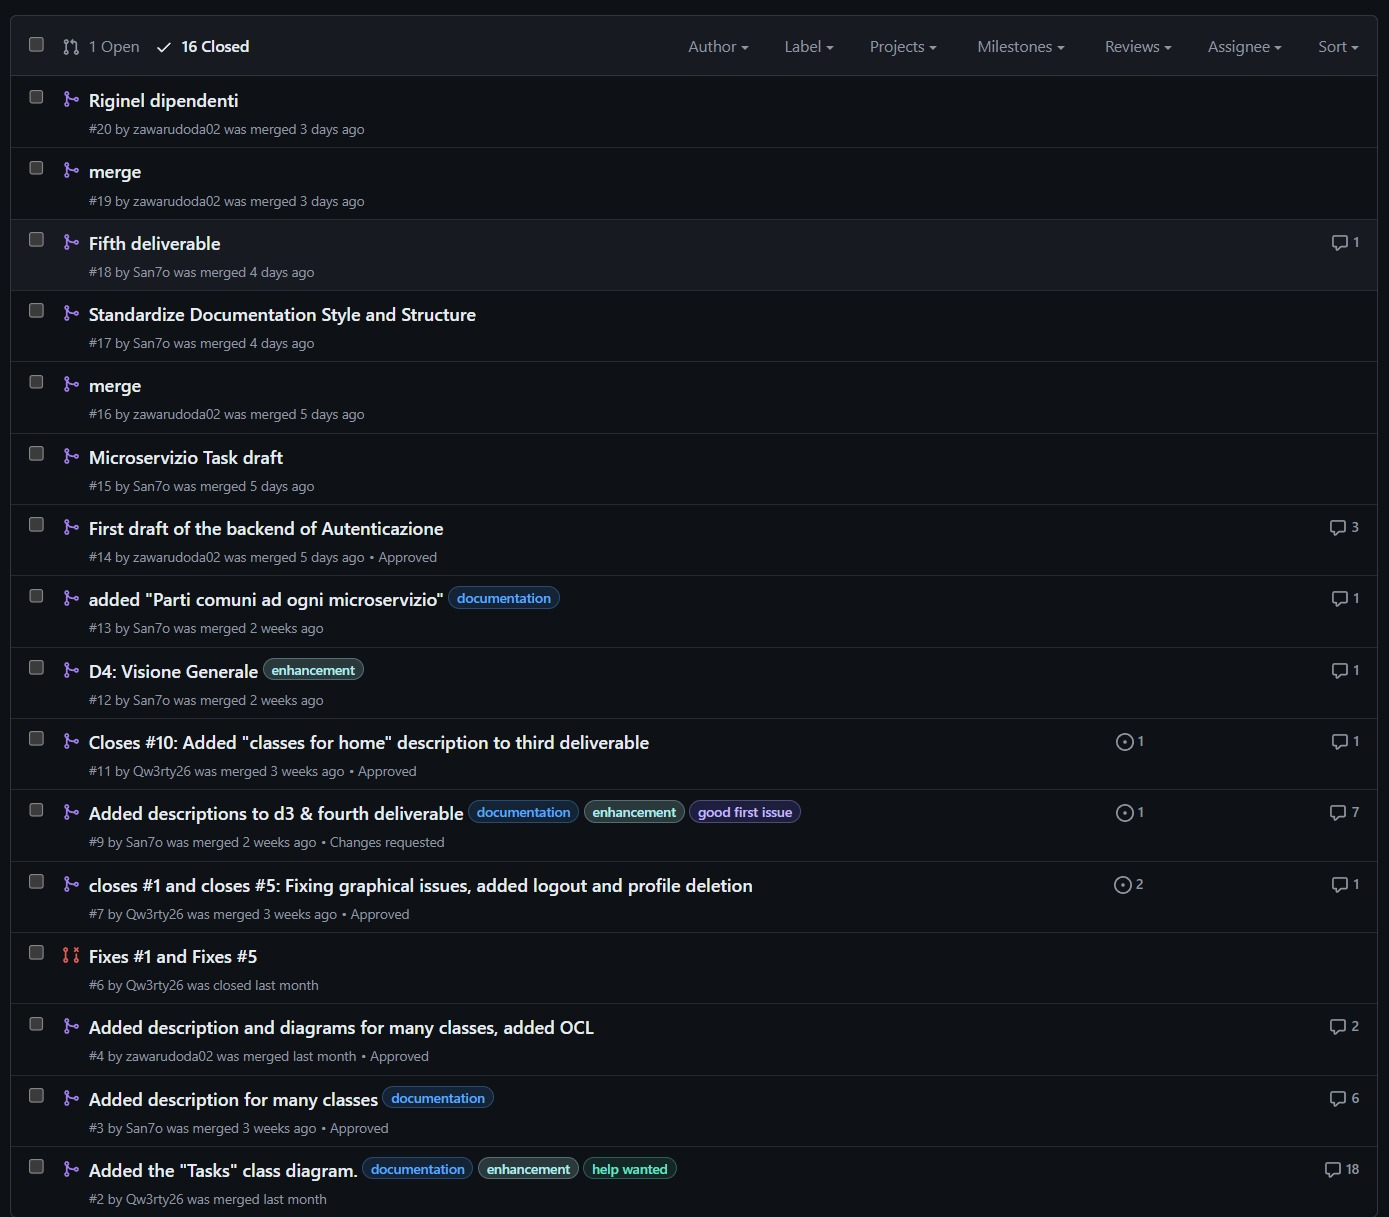
\includegraphics[width=1\textwidth]{images/github-image2.jpg}
	    	\caption{Pull Requests della repository "Documentation Source" su GitHub}
	    \end{figure}	
	\end{itemize}
	\item Google Drive
	\begin{itemize}
		\item Software per la memorizzazione e la sincronizzazione dei files
	\end{itemize}
	\item Draw.io
	\begin{itemize}
		\item Software per la creazione e lo sviluppo di diagrammi
		\begin{figure}[H]
			\centering
			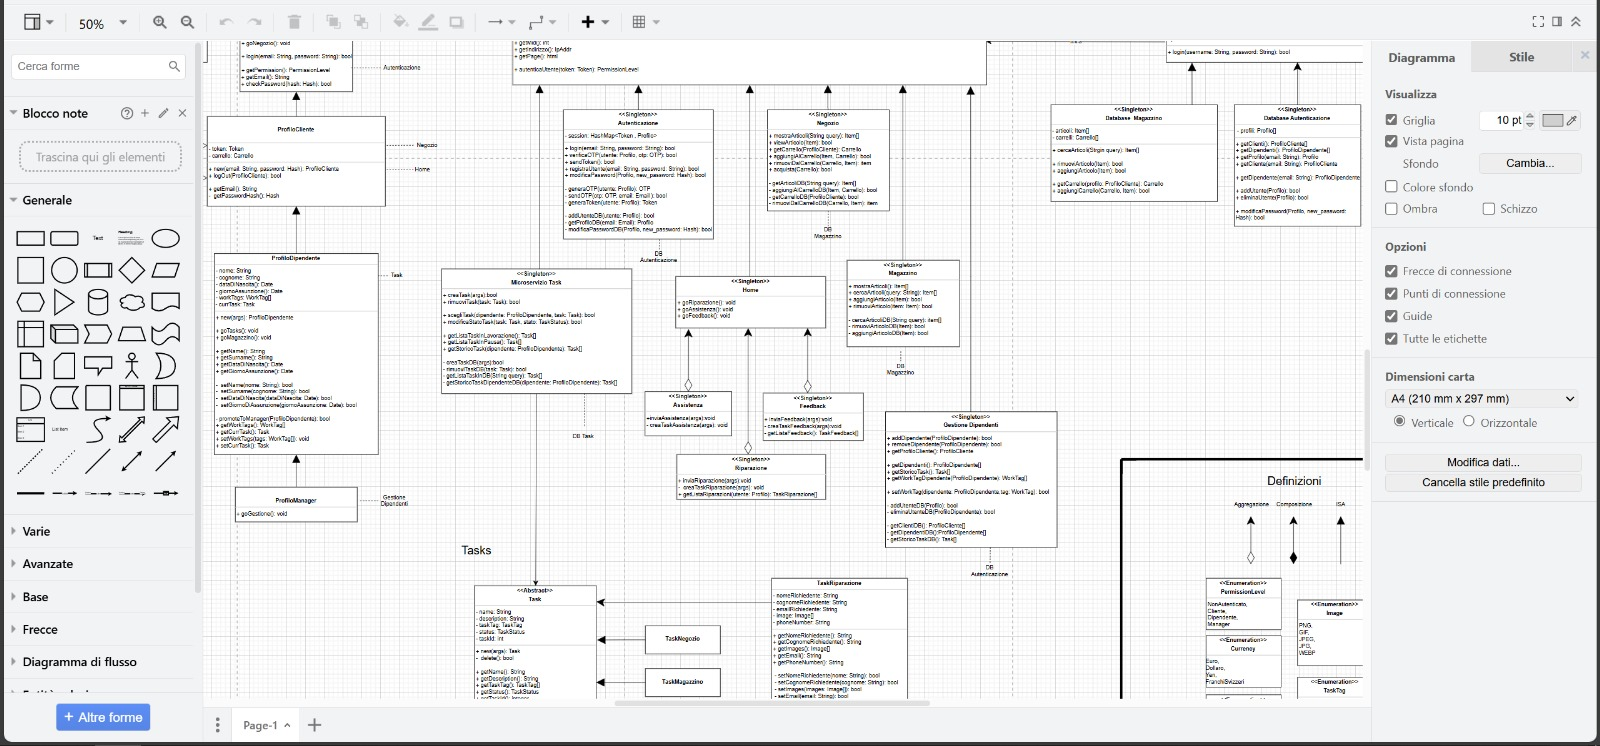
\includegraphics[width=1\textwidth]{images/drawio-image.jpg}
			\caption{Realizzazione del "Diagramma delle Classi" del third-deliverable}
		\end{figure}	
	\end{itemize}
	\item LaTeX
	\begin{itemize}
		\item Un linguaggio MarkUp specializzato nella realizzazione e scrittura di documenti di alta qualità.
		\begin{figure}[H]
			\centering
			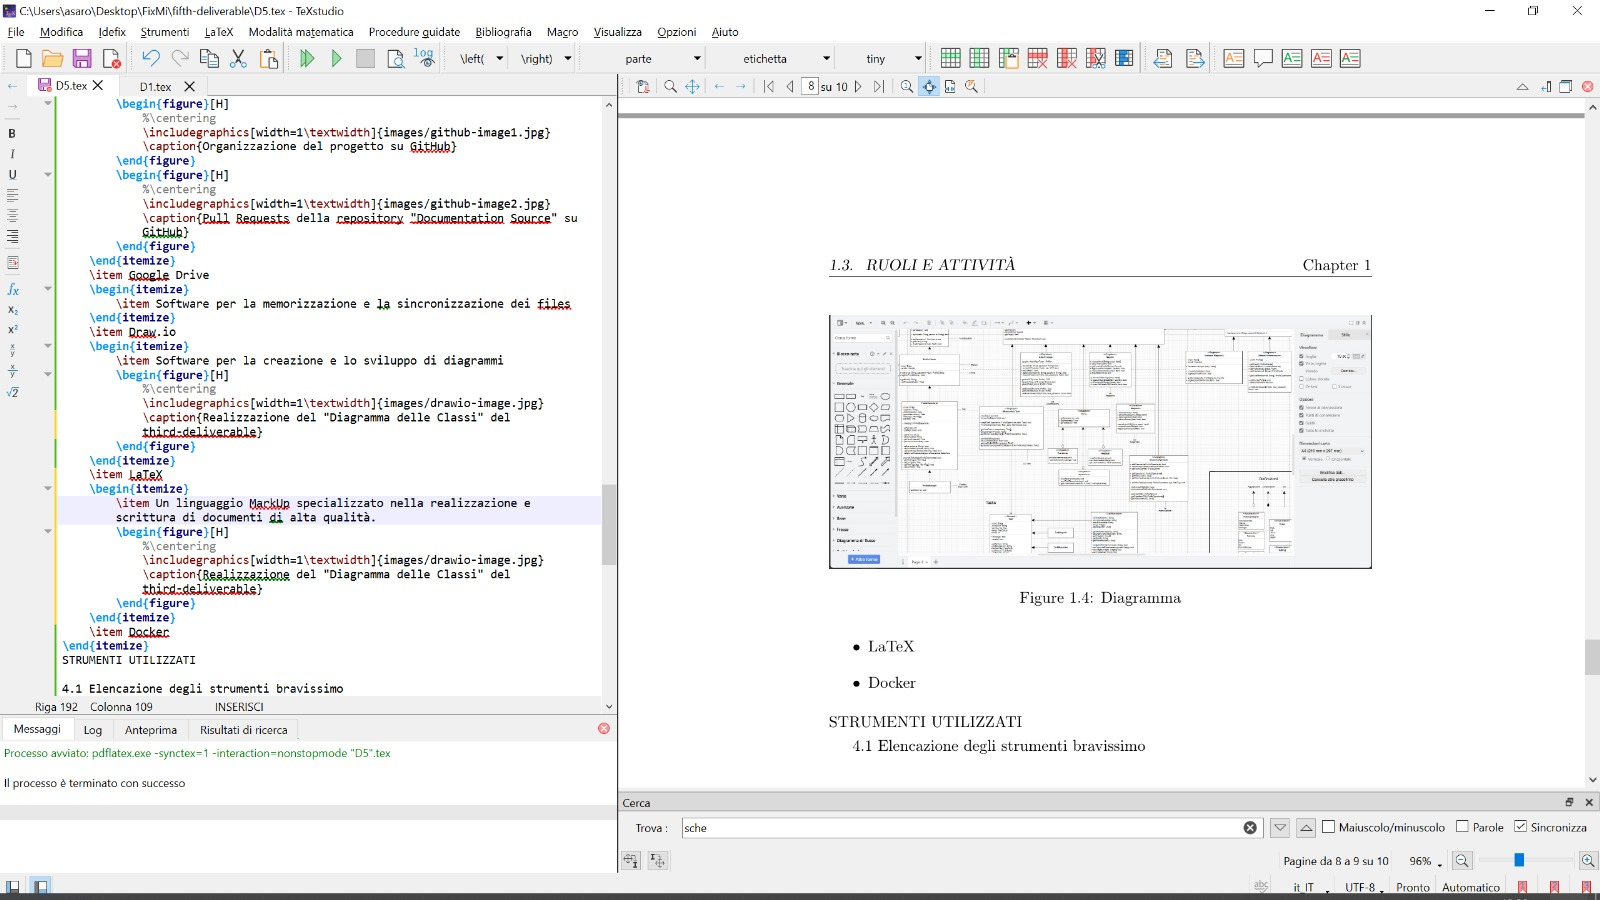
\includegraphics[width=1\textwidth]{images/latex-image.jpg}
			\caption{Scrittura del documento con LaTeX}
		\end{figure}	
	\end{itemize}
	
	\item Docker
	\begin{itemize}
		\item Software per l'esecuzione di processi e programmi in ambiente isolato tramite contenitori minimali e facilmente distribuibili.
		\begin{figure}[H]
			\centering
			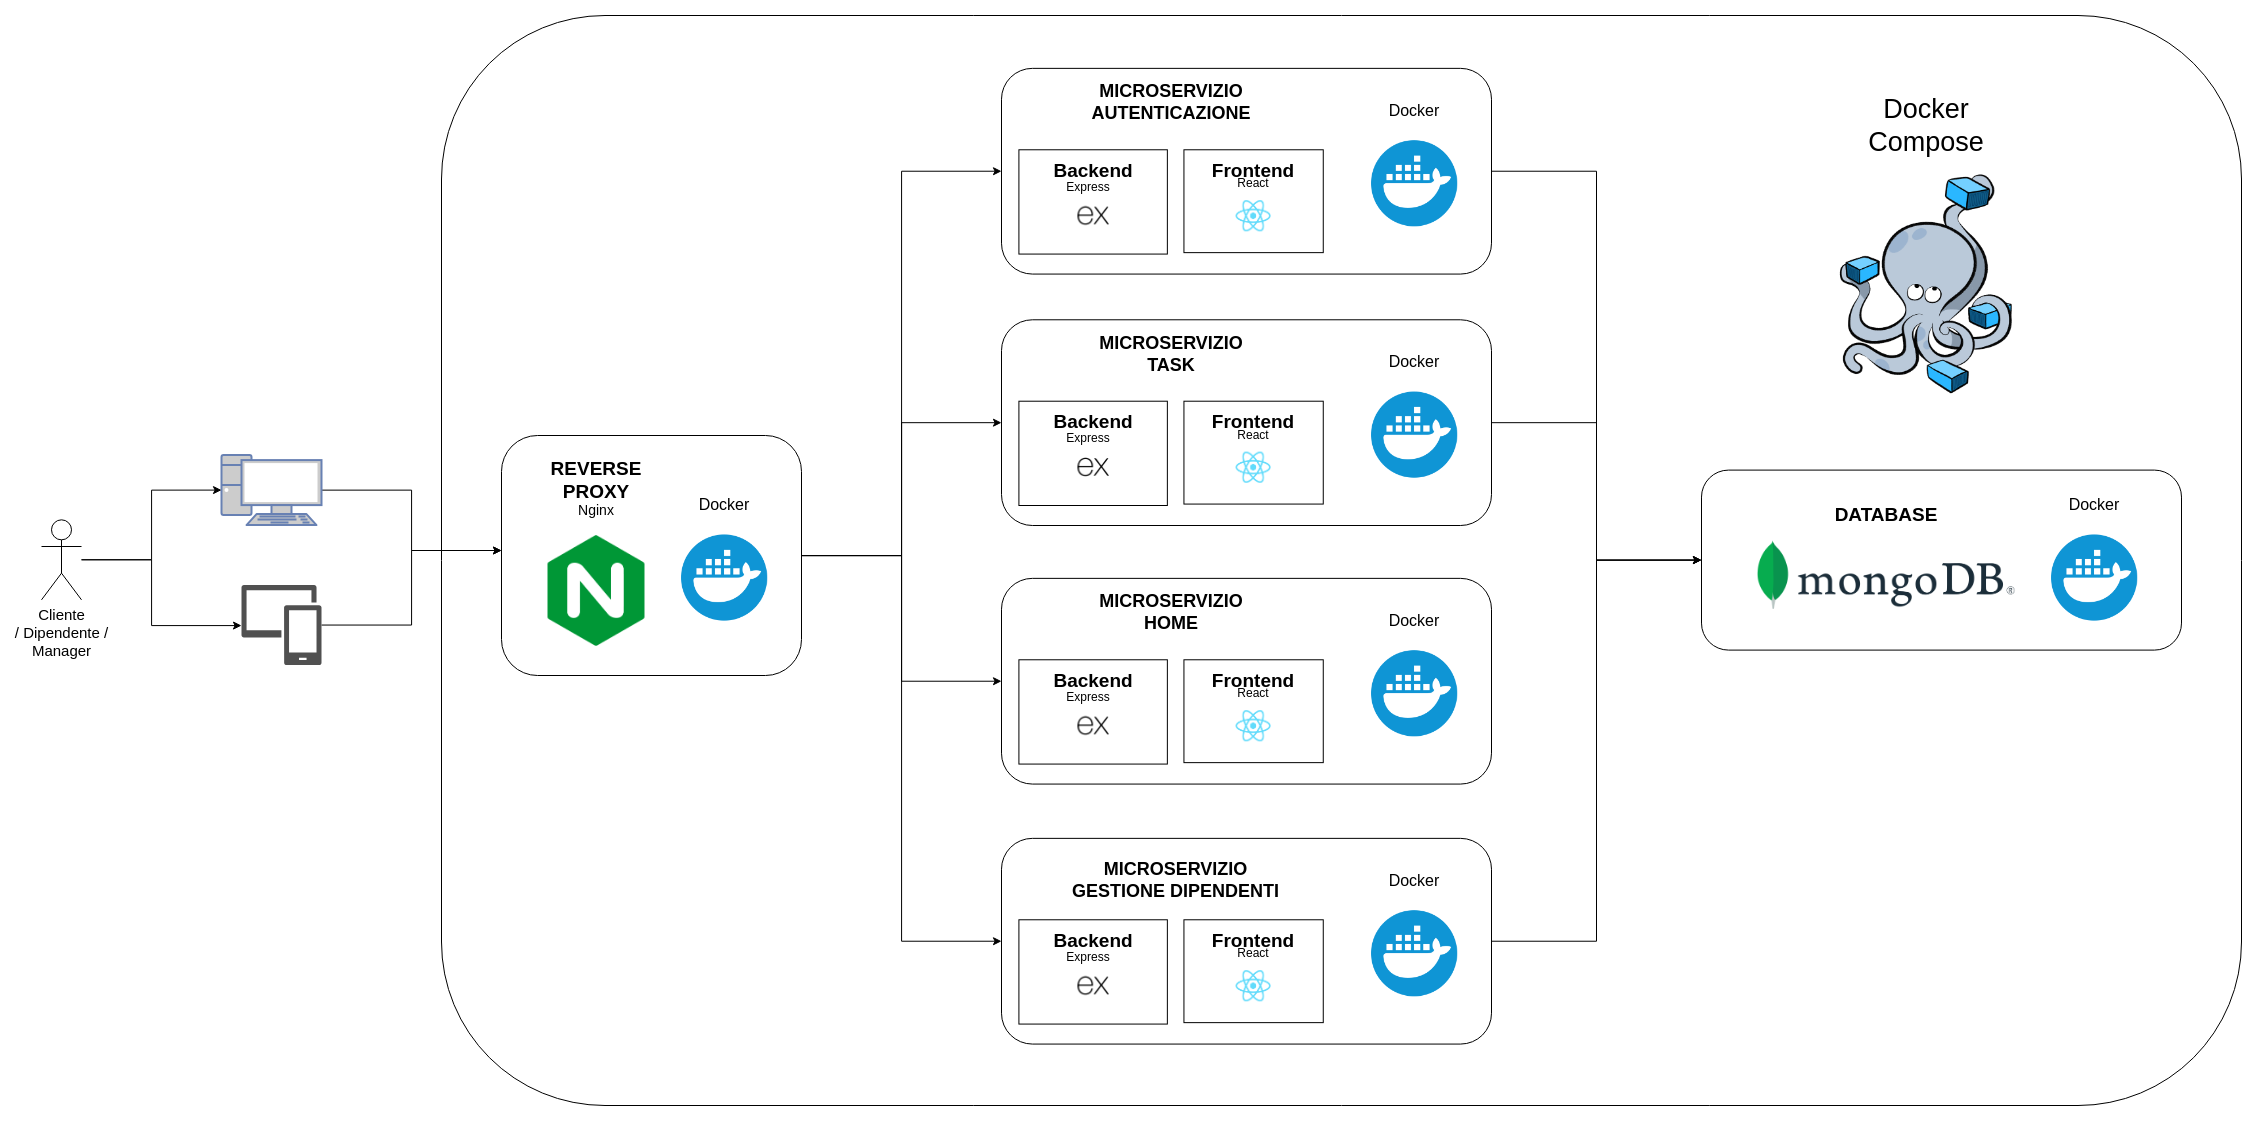
\includegraphics[width=1\textwidth]{images/diagramma_microservizi.png}
			\caption{Struttura del progetto tramite Docker}
		\end{figure}	
	\end{itemize}
	
\end{itemize}



\section{Ruoli e Attività}
% table
%table
\subsubsection{Riginel Ungureanu}
\begin{itemize}
	\item \textbf{Ruolo}: Leader del gruppo
	\item \textbf{Principali Attività}: Il membro ha coordinato il team durante il progetto, ha realizzato in particolar modo il sistema di autenticazione, ha contribuito attivamente alla documentazione e alla progettazione dell'applicazione.
\end{itemize}

\subsubsection{Giovanni Santini}
\begin{itemize}
	\item \textbf{Ruolo}: Responsabile Back-End
	\item \textbf{Principali Attività}: Il membro del team ha partecipato laboriosamente all'intero design e sviluppo dell'applicazione. In particolare, ha guidato il team durante la stesura del D3 e D4, si è occupato dell'infrastruttura e implementazione dei microservizi utilizzando tecnologie come Docker e Nginx; ha contribuito attivamente alla documentazione.
\end{itemize}


\subsubsection{Valerio Asaro}
\begin{itemize}
	\item \textbf{Ruolo}: Responsabile Front-End e Designer
	\item \textbf{Principali Attività}: Il compito principale è stato la realizzazione della parte Front-End dell'applicazione ma ha anche contribuito alla stesura della documentazione e alla progettazione dell'applicazione.
\end{itemize}

\section{Carico e distribuzione del lavoro}
Di seguito una tabella rappresentativa della distribuzione del carico lavorativo.
% table
\begin{center} % center the table
	\centering
	\begin{tabular}{ |p{3cm}|p{1cm}|p{1cm}|p{1cm}|p{1cm}|p{1cm}|p{1cm}|  }
		\hline
		\centering  Membri  &  D1 &  D2 & D3 & D4 & D5 & TOT\\ % I found no other way...
		\hline
		\centering Giovanni Santini & 39 & 22 & 30 & 108 & 5 & 204 \\ % I found no other way...
		\hline
		\centering Riginel Ungureanu & 26 & 37 & 21 & 84 & 8 & 176 \\ % I found no other way...
		\hline
		\centering Valerio Asaro & 21 & 16 & 17 & 54 & 5 & 113 \\ % I found no other way...
		\hline
		\centering TOT & 86 & 75 & 68 & 246 & 18 & 493 \\ % I found no other way...
		\hline
	\end{tabular}
\end{center}

\section{Criticità}
Il team di sviluppo ha trovato difficoltà nell'organizzare il proprio tempo, in particolar modo all'inizio del progetto. Il gruppo, non avendo esperienza pregressa nel design e lo sviluppo di software di questa scala, ha riscontrato complicazioni nella scrittura della documentazione e nell'apprendimento delle tecnologie utilizzate per la realizzazione dell'applicazione.

\section{Autovalutazione}
In definitiva il gruppo è molto soddisfatto del lavoro compiuto. Nonostante le criticità precedentemente descritte siamo riusciti a raggiungere i nostri obiettivi.
Segue la tabella dell'autovalutazione di ciascun membro del gruppo.
% table
\begin{center} % center the table
	\centering
	\begin{tabular}{ |p{3cm}|p{1cm}|  }
		\hline
		\centering  Membri  & Voto\\ % I found no other way...
		\hline
		\centering Giovanni Santini & 30L \\% I found no other way...
		\hline
		\centering Riginel Ungureanu & 30  \\% I found no other way...
		\hline
		\centering Valerio Asaro & 30  \\% I found no other way...
		\hline
	\end{tabular}
\end{center}



	
\end{document}